\documentclass[seminar]{plai}
\usepackage{tikz,pgfplots,amssymb,hyperref,float,setspace}
\usetikzlibrary{positioning,arrows.meta,calc}
\usetikzlibrary{graphs}

\usepackage{tabularx}

\usepackage{lipsum}

\title{VEX vs. P-Code: Intermediate Representations in the Reverse-Engineering Platforms angr and Ghidra}
\seminar{Proseminar Software-Hardening}
\author{Marcel Fiedler}
\matrikelnummer{777}
\semester{SoSe 2025}
\email{maximilian.mustermann@campus.lmu.de}


%%%%%%%%%%%%%%%%%%%%%%%%%%%%%%%%%%%%%%%%%%
\begin{document}

\maketitle

\begin{abstract}

\noindent Comparing binaries from different platforms and architectures is a necessary but complicated task in software hardening and malware analysis. Intermediate Representation offers a way of representing programming logic by rewriting it into an abstraction between the source language's structure and the target assembly's concrete structure, while detached from the limitations of an actual architecture. Reverse engineering platforms and compilers use it to further analyze it, such as optimization, analysis, and efficient code generation.

This approach also enables a better development of novel solutions: It is often easier and faster to create a lifter into an IR for a new architecture than to write an individual virtual machine for it.

\noindent This paper compares the IR of the popular reverse engineering platforms VEX from angr and p-code from Ghidra.
The focus lies on the different approaches of the IR, their creation and usage by the reverse engineering platforms, and their performance with varying analysis approaches.
\end{abstract}

%%%%%%%%%%%%%%%%%%%%%%%%%%%%%%%%%%%%%%%%%%
\section{Introduction}
\label{sec:introduction}

The term reverse engineering originates from hardware analysis, which aims to decipher the architecture of established products.\cite{reverse-engineering-design-recovery-taxonomy}\\
The reverse engineering process of software is the identification of the components of the system and their collaboration. The next step is to create an abstract representation of the system: The Intermediate Representation (IR).

Reverse engineering platforms and compilers use it to do further analysis, such as optimization, analysis, and code generation into higher-level languages such as C.

Intermediate representations, also known as intermediate languages, are designed to remove this burden.

IR offers a way of representing programming logic by rewriting it into an abstraction between the structure of the high-level language source and the concrete structure of the target assembly, while being detached from the limitations of an actual architecture.

Concrete assembly instruction sets contain complex semantics with different side effects, such as setting status flags.
The overwhelming quantity of those instructions makes automatic binary analysis complicated.

\noindent The use of IR offers more flexibility and saves time. It can also be used in a broader range of tools as an interface for many other binary analyses on top of the translated code. Instead of writing a specific handler for every binary analysis for each architecture, it only has to be done once using IR as a translation.

\noindent Reverse engineering offers a way to understand binary code from other authors and decide whether they are malicious or not, and as an offensive practice, develop methods to protect operating systems and crucial software against those attacks.

However, as the influence of technology widens even further and with an increasing usage of computer-driven tools in all aspects of industries and private lives in sight, the possibilities for software exploitation rise, as more and more of everyday life and critical infrastructure become influenced by computers.

Malware authors adapt to defense techniques with new attacks, crafting even more complicated ways of exploitation and making the binaries obfuscated to evade detection during the analysis process. These practices are called anti-disassembly: Code and data in programs are causing disassembly analysis to make incorrect program listings to veil the malicious intention of the program. Malware authors also use anti-disassembly techniques to disrupt the analysis process of malicious code; some of these techniques are: anti-disassembly, anti-debugging, anti-virtual machine techniques, and binary packing. \cite{practical-malware-analysis}
The variety of anti-reverse engineering techniques illustrates the need for further research and development in reverse engineering.

%%%%%%%%%%%%%%%%%%%%%%%%%%%%%%%%%%%%%%%%%%
\section{Background}
\label{sec:background}

\subsection{What is Reverse Engineering?}
\label{sec:reverse-engineering-background}
Software reverse-engineering is the analysis of systems in order to identify their components and their interrelationships. Furthermore, to represent the system in another form or abstraction.\cite{reverse-engineering-design-recovery-taxonomy}
The IEEE Standard for Software Maintenance defines reverse engineering as "the process of extracting software system information from source code."\cite{ieeeStandard-for-SW-maintenance}
It can, however, start at any level of abstraction and any stage of the software development life cycle. The goal of the examination is to understand the logic behind a program and decide whether it is harmful. The main domains of reverse engineering are \textit{redocumentation} and \textit{design recovery}.
\\\\
\textbf{Redocumentation}\\
Redocumentation is the recreation of a "semantically equivalent representation within the same relative abstraction level"\cite[p.15]{reverse-engineering-design-recovery-taxonomy}, e.g., dataflow, data structures, control flows, for a better oversight.
It is the simplest and oldest form of reverse engineering. The goal is to provide an easily understandable visual documentation of the program components.\cite{reverse-engineering-design-recovery-taxonomy}
\\\\
\textbf{Design recovery}\\
Design recovery is the gaining of insights of higher-level abstractions beyond the direct observation itself by combining domain- and external information, as well as domain knowledge or fuzzy reasoning.\cite{reverse-engineering-design-recovery-taxonomy}
\\\\
\textbf{Restructuring}\\
Restructuring means changing one form of representation into another on the same level of abstraction, all while preserving the behavior of the software.\cite{reverse-engineering-design-recovery-taxonomy}
\\\\
\textbf{Reengineering}\\
Reengineering is the analysis of a program to alter it into a new form.

\subsection{Disassembly vs. Decompilation}
\label{disassembly-vs-decompilation}

\textbf{Disassembling}\\
Reverse engineering with disassembly is the translation of binaries in machine code into human-understandable assembly
One of the caveats of the faster execution of \textit{compiled languages} in comparison to interpreted ones is the loss of meta-information from the original program, e.g., lost names of variables and functions; therefore, complete reversion is impossible.
However, a disassembler can trace back the execution and display it as human-readable assembly.\cite{reverse-engineering-vs-disassembly}\\

\begin{figure}[htbp]
\centering
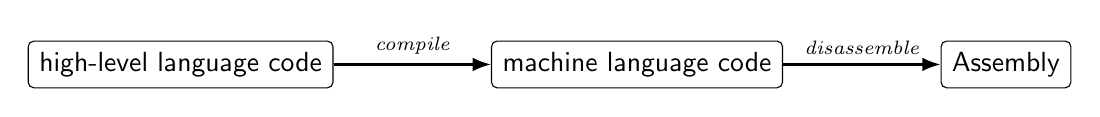
\begin{tikzpicture}[
  font=\sffamily,
  block/.style={draw, rounded corners=2pt, align=center, inner sep=4pt},
  arr/.style={-Latex, thick},
  note/.style={font=\itshape\scriptsize, midway, above}
]

% nodes
\node[block] (high) {high-level language code};
\node[block, right=of high, xshift=10mm] (machine) {machine language code};
\node[block, right=of machine, xshift=10mm] (assembly) {Assembly};

% arrows with labels
\draw[arr] (high) -- node[note] {compile} (machine);
\draw[arr] (machine) -- node[note] {disassemble} (assembly);

\end{tikzpicture}
\caption{Disassembly workflow\cite{reverse-engineering-vs-disassembly}}
\label{fig:compile-disassemble}
\end{figure}

\noindent\textbf{Decompile}\\
\textit{Interpreted languages} such as Java and Python are not compiled into machine code, but into \textit{bytecode}, which gets interpreted at runtime by a virtual machine. Despite some optimization and restructuring, the context is still preserved, which makes the reverse translation into the original high-level language code possible.\cite{reverse-engineering-vs-disassembly}

\begin{figure}[htbp]
\centering
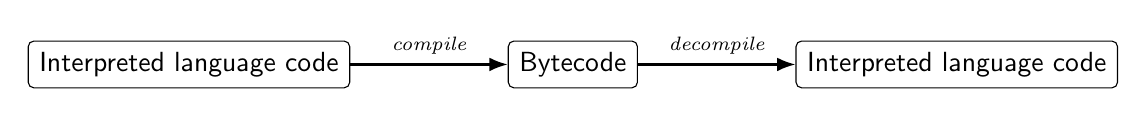
\begin{tikzpicture}[
  font=\sffamily,
  block/.style={draw, rounded corners=2pt, align=center, inner sep=4pt},
  arr/.style={-Latex, thick},
  note/.style={font=\itshape\scriptsize, midway, above}
]

% nodes
\node[block] (interp1) {Interpreted language code};
\node[block, right=of interp1, xshift=10mm] (bytecode) {Bytecode};
\node[block, right=of bytecode, xshift=10mm] (interp2) {Interpreted language code};

% arrows with labels
\draw[arr] (interp1) -- node[note] {compile} (bytecode);
\draw[arr] (bytecode) -- node[note] {decompile} (interp2);

\end{tikzpicture}
\caption{Decompilation workflow\cite{reverse-engineering-vs-disassembly}}
\label{fig:interpret-bytecode}
\end{figure}


\subsection{Platforms for Reverse Engineering and Binary Analysis}
\label{sec:platforms-for-reverse-engineering-binaryAnalysis-background}
Binary analysis is the most important reverse engineering practice: Examining binaries to uncover vulnerabilities and threats when the original high-level language source code is unavailable.
Security specialists and researchers developed a variety of platforms for binary analysis and other reverse engineering techniques that offer an efficient and professional way of analyzing binaries.

\subsection{Intermediate Representations}
\label{sec:ir-background}
Intermediate Representations are used internally by compilers, decompilers, and virtual machines.
IR translates the machine code of concrete architectures into a more abstract representation of its program logic.
It is used for optimization, analysis, and efficient code generation. An \textit{external format} of IR may be used as an interface for other unrelated tools that enable reverse-engineering platforms.
There are many types of IR. This term paper will present the \textit{static single assignment form} and the \textit{Register Transfer Language}.\\

\noindent\textbf{Static Single Assignment (SSA)}\\
It is a commonly used form for IR with static variables, commonly used for complex optimizations. The variables in the code blocks of the control flow graph have the restriction that they cannot be updated. Instead, a new version replaces the variable\cite{introduction-to-compilers-and-language-design}: The left side of every variable assignment must have a unique name. An individual $\phi$-function determines the output of each basic code block. It computes a result based on the input operands, which are selected on the basis of the control flow edge through which the dynamic execution entered the block.\cite{interpreting-programs-in-SSA-form}\\


\noindent\textbf{Register Transfer Language (RTL)}\\
RTLs are a low-level IR, often used by compilers for optimization.\\
It forms machine instructions by combining as many logical statements as possible without simplifying them by breaking them down.\\
RTL models computations of the actual hardware as operations that transfer values between virtual registers and memory.
\cite{The-RTL-System-A-Framework-for-Code-Optimization}\\

\noindent\textbf{Control Flow Graph (CFG)}\\
Another important IR type is CFG, which shows the higher-level structure of a program. CFGs are directed graphs whose nodes are \textit{basic blocks}, i.e., maximal sequences of statements with a single entry and single exit.
The edges between them represent the decision flow of sequential execution. Conditional constructs appear as separate blocks and result in branch nodes in the graph that split the control flow, while cycles represent loops in the graph.
\cite{introduction-to-compilers-and-language-design}

%%%%%%%%%%%%%%%%%%%%%%%%%%%%%%%%%%%%%%%%%%
\section{Reverse Engineering Internals}
\label{sec:reverse-engineering-internals}

\subsection{angr internals}
\label{sec:angr-internals}

The first step into reverse-engineering with angr is loading a binary into a project, which consists of information about its CPU architecture, filename, and the entry point address.\cite{core-concepts} The binary is then loaded into the angr analysis system by the \textit{CLE loader} by providing base classes for reproducing binary objects.
CLE uses file format parsing libraries, e.g., elftool for Linux and portable executable files for Windows, to parse the objects themselves.
Then the \textit{memory image} is exposed by relocations in the binary file.\cite{art-of-war-angr}
The \texttt{SimuVEX} module creates a \textit{program state}, a snapshot of registers, memory, and open files, which is then used by angr's simulation engine \texttt{SimEngine}.

\texttt{The SimuVEX} module creates a program state and a snapshot of registers, memory, and open files, which is then used by angr's simulation engine, SimEngine. SimuVEX uses a set of plugins, such as \texttt{project.factory.block()}, to extract basic blocks from the binary into block objects, which saves the entry point of the code block, assembly mnemonics, an instruction counter, as well as addresses of the instructions.\cite{art-of-war-angr} This data is then used as abstract expressions in an expression tree with values as leaf nodes and operations as non-leaf nodes.\\

Claripy's functionality is made up of two parts: the \textit{front end} and the \textit{back end}. The backend can translate the expressions into data domains during the examination process. It supports the concrete domain (integers, floating-point numbers) and the symbolic domain (symbolic integers and floating-point numbers).
The frontend modules augment the backend with additional functionality, such as \textit{symbolic solving, constraint solving, expression interpretation, and symbolic constraint solving}.
angr provides several analyses, e.g., \textit{dynamic symbolic execution} and \textit{CFG recovery}. The primary interfaces for such analyses are \texttt{path groups}, modules that are interfaces to dynamic symbolic execution. They track execution paths of applications. \texttt{Analyses} provide abstractions for complete program analyses and manage static analyses.


\begin{figure}[H]
%[htbp]
\centering
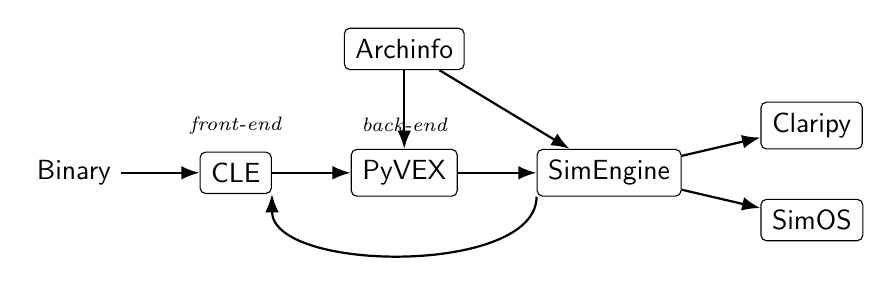
\begin{tikzpicture}[
  font=\sffamily,
  block/.style={draw, rounded corners=2pt, align=center, inner sep=4pt},
  arr/.style={-Latex, thick},
  note/.style={font=\itshape\scriptsize}
]

% nodes
\node (bin) {Binary};
\node[block, right=of bin] (cle) {CLE};
\node[note, above=0.1cm of cle] {front-end};

\node[block, right=of cle] (pyvex) {PyVEX};
\node[note, above=0.1cm of pyvex] {back-end};

\node[block, right=of pyvex] (sim) {SimEngine};

\node[block, above=of pyvex] (arch) {Archinfo};

\node[block, right=of sim, yshift=6mm] (claripy) {Claripy};
\node[block, right=of sim, yshift=-6mm] (simos) {SimOS};

% arrows
\draw[arr] (bin) -- (cle);
\draw[arr] (cle) -- (pyvex);
\draw[arr] (pyvex) -- (sim);
\draw[arr] (arch) -- (pyvex);
\draw[arr] (arch) -- (sim);
\draw[arr] (sim) -- (claripy);
\draw[arr] (sim) -- (simos);

% curved dependency from SimEngine back to CLE
\draw[arr] (sim.south west) .. controls +(0,-1.0) and +(0,-1.0) .. (cle.south east);

\end{tikzpicture}
\caption{Internal workflow of angr.\cite{angr-internals}}
\label{fig:angr-flow}
\end{figure}

\noindent\textbf{CLE loader}\\
The CLE loader (CLE stands for "CLE loads everything") extracts the actual executable from the binary code. It can read many types, such as portable executable, executable, and linking format binaries.
The CLE loader is a set of \textit{binary objects} loaded and mapped into a single memory space. A specialized loader backend processes each file type. Depending on the header of the file, CLE then makes assumptions about the intended architecture of the binary. It creates a representation of the \textit{memory map}, and the virtual memory segment is assigned a direct byte-for-byte correlation with some part of the file by simulating the actual loader. The result is a Loader object with the memory of the program.\cite{loading-a-binary}\\

\textbf{Archinfo}\\
During the loading process, an analysis evaluates the header and other heuristics to guess the targeted architecture of the binary file. The \texttt{archinfo} library gets called with this information and returns a map of the register file, bit width, usual endian-ness, etc.\\

\textbf{SimEngine}\\
The SimEngine interprets the code in a meaningful way. It saves the \textit{program's state}, a snapshot of the registers, memory, basic block of instructions, etc., and produces a set of \textit{successors}: Possible data program states that can be reached from this block.
The constraints and conditions needed to take the branches' paths are collected when branches occur.\\

\textbf{PyVEX}\\
The default engine of the lifter, \texttt{SimEngineVEX}, supports many architectures because it does not run directly on their machine code. Instead, it uses the \texttt{VEX IR}, which the machine code is lifted into.\cite{angr-internals}\\
Instead of creating a new engine for a special architecture, a lifter can be a more efficient solution: It allows PyVEX to take care of the rest.\cite{art-of-war-angr}\\

\textbf{Claripy}\\
Angrs lifter Claripy is an abstracted constraint-solving wrapper.\cite{claripy-documentation} Operations are not represented as concrete values, but as expressions that are eventually composed from several expressions. Claripy creates these compositions and solves them with Microsoft's SMT-solver Z3.\cite{angr-internals}

\textbf{SimOS}\\
The OS provides higher-level functionality and abstraction, such as \texttt{stdin}, file management, and networking. SimOS provides an abstraction for this by defining OS-specific embellishments on the initial state of the program. The \texttt{SimProcedures} module provides \texttt{system calls} and symbolic summaries of syscalls and standard library functions.
This makes angr faster and compatible than symbolically executing \texttt{libc} itself.


\subsection{Ghidra internals}
\label{sec:angr-internals}
\begin{figure}[htbp]
\centering
\resizebox{\textwidth}{!}{%
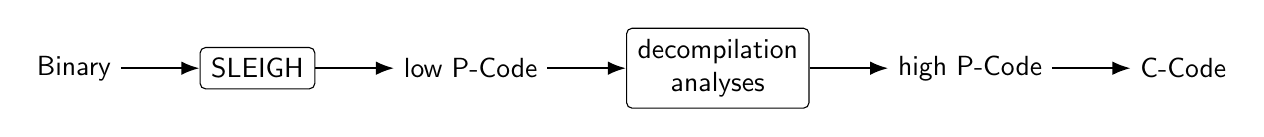
\begin{tikzpicture}[
  font=\sffamily,
  block/.style={draw, rounded corners=2pt, align=center, inner sep=4pt},
  arr/.style={-Latex, thick}
]

% nodes
\node (bin) {Binary};
\node[block, right=of bin] (sleigh) {SLEIGH};
\node[right=of sleigh] (lowp) {low P-Code};
\node[block, right=of lowp] (decomp) {decompilation\\analyses};
\node[right=of decomp] (highp) {high P-Code};
\node[right=of highp] (ccode) {C-Code};

% arrows
\draw[arr] (bin) -- (sleigh);
\draw[arr] (sleigh) -- (lowp);
\draw[arr] (lowp) -- (decomp);
\draw[arr] (decomp) -- (highp);
\draw[arr] (highp) -- (ccode);

\end{tikzpicture}%
}
\caption{Internal Ghidra workflow.\cite{formal-semantics-for-P-Code}}
\label{fig:ghidra-flow}
\end{figure}

\noindent The first step of the Ghidra reverse engineering process is the binary disassembly with \textit{SLEIGH}.\cite{formal-semantics-for-P-Code}\\
SLEIGH is a \textit{processor specification language} for Ghidra. It is derived from \textit{SLED (specification language for encoding and decoding)}.
It is a language for describing an instruction set of general-purpose microprocessors and detailed enough to facilitate the \textit{disassembly-} and \textit{decompilation engines}.\\
For disassembly, SLEIGH offers a concise description of the translation from bit encoding of the machine instructions to readable assembly code. The single operands get divided into mnemonic operands, sub-operands, and associated syntax.\cite{sleigh-a-language-for-rapid-processor-specification}\\
As for the decompilation, SLEIGH describes the rules for the translation from machine instructions into p-code.
It describes the specification of the encoding for processors with \texttt{.slaspec}-files.\cite{sleigh-a-language-for-rapid-processor-specification, ghidra-book-definite-guide}

%%%%%%%%%%%%%%%%%%%%%%%%%%%%%%%%%%%%%%%%%%
\section{Comparison of the IR types}
\label{sec:comparison-of-the-ir-types}

\subsection{VEX}
Julian Seward developed the VEX IR (Virtual Execution eXtended Intermediate Representation) as a part of \textit{Valgrind} in 2000 as a memory debugging tool. However, it has since evolved into a modular framework for binary analysis for various architectures. 
Its core design is dynamic binary translation, which allows the analysis of every instruction executed in a program. In contrast to angr, which uses the VEX IR for \textit{static-} and \textit{dynamic symbolic execution}, \textit{CFG-recovery} and \textit{vulnerability detection}.
Valgrind focuses on runtime correctness checking and profiling.
angr is designed for program reasoning, reverse engineering, and automated exploit discovery as a broader, more research-oriented development process. VEX IR represents register content as separate memory spaces with integer offsets, enables memory segmentation, and is free of side effects. It represents the functionality of processors as four objects: \textit{expressions, operations, temporary variables, statements}, and \textit{blocks}.\cite{Valgrind-A-Framework-for-Heavyweight-Dynamic-Binary-Instrumentation}\\

\noindent\textbf{Expressions}\\
Content of memory and registers and their results of \textit{IR operations}.\\

\noindent\textbf{Operations}\\
IR Operation represents the modifications on the IR expression-values.
The data types include integers, arithmetic, floating-point numbers, bit-operations.\\

\noindent\textbf{Temporary variables}\\
Data may be stored as strongly typed temporary variables in \textit{internal registers}, which can be read with IR operations.\\

\noindent\textbf{Statements}\\
IR Statements keep track of changes in the state of the targeted processor architecture, such as read and write in memory and registers. The data that they use is retrieved by the IR expressions.\\

\noindent\textbf{Blocks}\\
IR blocks represent \textit{IR super blocks (IRSB)} of the targeted architecture and are a set of IR statements.

\subsection{P-Code}
 Ghidra uses \textit{p-code} as IR. It is a \textit{register transfer language} \cite{PCode-reference-manual} general enough to abstract the machine code of several general-purpose processors. It enables explicit data manipulation on user-defined registers and address spaces. During the analysis process, the p-code also gets lifted into \textit{single static assignment (SSA)}\cite{working-with-ghidras-pCode-to-identify-vulnerable-function-calls}. During the SSA optimization, all code blocks get updated with data gained from the analysis of the control flow. However, whenever the value of a variable changes, it does not get updated; instead, it is replaced by a new version number.\cite{introduction-to-compilers-and-language-design}
P-Code mirrors processor tasks and concepts with three core ideas: \textit{Address space, Varnodes} and \textit{Operations}.\\

\noindent\textbf{Address Spaces}\\
The p-code address space is a generalization of RAM.
It is defined as a sequence of bytes that can be read and written by p-code operations and is characterized by name and size. Only in the address spaces can data be manipulated.\\

\noindent\textbf{Varnodes}\\
Registers of a processor are represented by varnodes. They are saved as a continuous set of bytes in a p-code address space and get manipulated by p-code operations.
Varnodes are typeless sequential bytes, only characterized by a starting address and size. The p-code operations can then interpret them as types, which are integer, boolean, and floating point numbers.\\

\noindent\textbf{Operations}\\
P-Code operations represent the machine instructions of a processor.
All operations are mapped to the address of a specific machine instruction and can be generalized as functions which take one or more varnodes as input and exactly one varnode as output:\cite{PCode-reference-manual}
$$
\text{P-Code operation}(v_0,v_1,\dots,v_{n\in\mathbb N}) \rightarrow v_{new}
$$

\section{Performance comparison}
\label{sec:performance comparison}
VEX IR was developed by the valgrind project with an architecture-agnostic approach, focusing on abstraction and quick program analysis, which may be not human readable but optimized for automatization and symbolic execution.\\
p-code focuses mainly on static analysis and decompilation, and has a more human-readable semantics and a clearer mapping from machine code to IR with lower abstraction.\\
The following comparison is regarding the difference in performance measuring outcomes of the papers:\textit{ Decompilebench: A comprehnsible benchmark for evaluating decompilers in the real world scenarios}\cite{decompileBench-comprehensice-benchmark-for-evaluating-decompilers-in-real-world-scenarios}, \textit{DisCo: Combining Disassemblers for Improved Performance}\cite{DisCo-combining-disassemblers-for-improved-performance} and \textit{An Empirical Study on ARM Disassembly Tools}\cite{an-empirical-study-on-ARM-disassembly-disassembly-tools}

\subsection{Decompilation}
\texttt{DecompileBench} is the first comprehensible framework for effective evaluation of compilers in reverse engineering workflows, focusing on semantic accuracy and analyst usability of decompilation.\\
While the paper focuses on the possibility of the usage of LLM-powered approaches for reverse engineering, the takeaway for this seminar paper will be the IR benchmark comparisons.\\
\\
The \hyperref[sec:decompileBench-comparison]{table} below shows the \textit{recompile success rate (RSR)} and \textit{coverage equivalence rate (CER)} of angr and Ghidra with several compiler optimization stages.\\
The RSR is the percentage of decompiled functions that can be successfully recompiled back into valid machine code. It measures whether the output is able to compile. If the decompiler produces code that the compiler accepts and turns into an executable without errors, it counts as a success.\\
CER measures how many recompiled functions preserve the original behavior at runtime and produce an equivalent execution outcome.

\begin{table}[h]
\centering
\resizebox{\textwidth}{!}{%
\begin{tabular}{|l|c|c|c|c|c|c||c|c|c|c|c|c|}
\hline
 & \multicolumn{6}{c||}{\textbf{Recompile Success Rate}} & \multicolumn{6}{c|}{\textbf{Coverage Equivalence Rate}} \\
\hline
\textbf{Decompiler} & \textbf{O0} & \textbf{O1} & \textbf{O2} & \textbf{O3} & \textbf{Os} & \textbf{Avg} & \textbf{O0} & \textbf{O1} & \textbf{O2} & \textbf{O3} & \textbf{Os} & \textbf{Avg} \\
\hline
Angr   & 0.309 & 0.232 & 0.190 & 0.181 & 0.191 & \textbf{0.221} & 0.187 & 0.153 & 0.124 & 0.116 & 0.118 & \textbf{0.140} \\
\hline
Ghidra & 0.524 & 0.421 & 0.395 & 0.377 & 0.353 & \textbf{0.413} & 0.374 & 0.294 & 0.256 & 0.241 & 0.228 & \textbf{0.278} \\
\hline
\end{tabular}%
}
\caption{Comparison of Angr and Ghidra for Recompile Success Rate and Coverage Equivalence Rate.\cite{decompileBench-comprehensice-benchmark-for-evaluating-decompilers-in-real-world-scenarios}}
\label{sec:decompileBench-comparison}
\end{table}

\subsection{Disassembly}
In order to combine disassemblers, \texttt{DisCo} evaluates the performance of commonly used reverse engineering tools using \textit{Correctly identified function starts (CFS)} as well as \textit{precision and recall} and their derived F1 scores as key metrics for comparison of disassemblers.\\
angr outperforms at the disassembly of \texttt{MIPS}-binaries, where it has a $4.035\,\%$ better F1-score than Ghidra.
However, it performs worse than Ghidra with \texttt{}{ARM}-binaries.
\begin{table}[H]
\centering
\begin{tabular}{|l|c|c||c|c|}
\hline
 & \multicolumn{2}{c||}{\textbf{GCC}} & \multicolumn{2}{c|}{\textbf{Clang}} \\
\hline
\textbf{Disassembler} & \textbf{Average} & \textbf{5PWC} & \textbf{Average} & \textbf{5PWC} \\
\hline
\textbf{Angr}   & 82.0 & 71.5 & 86.8 & 77.3 \\
\hline
\textbf{Ghidra} & 76.8 & 57.2 & 85.3 & 70.1 \\
\hline
\end{tabular}
\caption{Comparison of Angr and Ghidra for GCC and Clang.\cite{DisCo-combining-disassemblers-for-improved-performance}}
\end{table}

\begin{table}[H]
\centering
\begin{tabular}{|l|c|c||c|c|}
\hline
 & \multicolumn{2}{c||}{\textbf{MIPS}} & \multicolumn{2}{c|}{\textbf{ARM}} \\
\hline
\textbf{Disassembler} & \textbf{GCC} & \textbf{Clang} & \textbf{GCC} & \textbf{Clang} \\
\hline
\textbf{Angr}   & 82.0 & 86.8 & 50.2 & 43.9 \\
\hline
\textbf{Ghidra} & 76.8 & 85.3 & 87.0 & 91.3 \\
\hline
\end{tabular}
\caption{Comparison of Angr and Ghidra for MIPS and ARM across GCC and Clang.}
\end{table}

\begin{table}[H]
\centering
\resizebox{\textwidth}{!}{%
\begin{tabular}{|l|c|c|c|c||c|c|c|c||c|c|c|}
\hline
\textbf{Tool} & \multicolumn{4}{c||}{\textbf{Instruction Boundary}} & \multicolumn{4}{c||}{\textbf{Function Boundary}} & \textbf{\#} \textbf{Timeout} & \textbf{\# Exception} & \textbf{\# Segfault} \\
\hline
 & \textbf{Precision} & \textbf{Recall} & \textbf{F1 Score} & \textbf{\# Invalid} & \textbf{Precision} & \textbf{Recall} & \textbf{F1 Score} & \textbf{\# Invalid} &  &  &  \\
\hline
\textbf{Angr}   & 0.886 & 0.797 & 0.830 & 1 & 0.404 & 0.667 & 0.490 & 1 & 16 & 364 & 262 \\
\hline
\textbf{Ghidra} & 0.954 & 0.828 & 0.873 & 0 & 0.855 & 0.714 & 0.766 & 0 & 13 & 0 & 0 \\
\hline
\end{tabular}%
}
\caption{Comparison of Angr and Ghidra on Instruction Boundary and Function Boundary metrics.\cite{an-empirical-study-on-ARM-disassembly-disassembly-tools}}
\end{table}


%%%%%%%%%%%%%%%%%%%%%%%%%%%%%%%%%%%%%%%%%%

%%%%%%%%%%%%%%%%%%%%%%%%%%%%%%%%%%%%%%%%%%

\section{Evaluation}
\label{sec:evaluation}

The benchmark comparison of the evaluated papers shows that Ghidra has, in almost all cases, a better performance than angr.\\
The only benchmark where angr outperforms Ghidra is the disassembly of \texttt{MIPS}-binaries from\texttt{GCC}- and \texttt{Clang} Compiler, where it has a $4.035\,\%$ better F1-score than angr on average.\cite{DisCo-combining-disassemblers-for-improved-performance}\\
Across the other performance metrics, Ghidra exhibits superior results compared to angr: In the \textit{DecompileBench}-paper, Ghidra outperforms angr by $49.64\,\%$ in decompilation.\cite{decompileBench-comprehensice-benchmark-for-evaluating-decompilers-in-real-world-scenarios}\\
In the \texttt{ARM}-comparison, Ghidra performs $4.92\,\%$ better at finding instruction boundaries and $36.01\,\%$ better at detecting function boundaries.\cite{an-empirical-study-on-ARM-disassembly-disassembly-tools}

%%%%%%%%%%%%%%%%%%%%%%%%%%%%%%%%%%%%%%%%%%
\section{Related Work}
\label{sec:related-work}
\textbf{DisCo: Combining Disassemblers for Improved Performance}\\
The \texttt{DisCo} (Disassembler Combination) project combines several industry-grade disassemblers into one novel open-source tool. It can be used to improve other disassemblers. \texttt{Ghidra+}, the improved version of Ghidra can achieve a 13,6\% better F1 score compared to the original. The paper also discovers a bug in Ghidra v9.1. The crucial takeaway for this comparison is that configuration has an important effect on disassembly performance: angr is the best among \texttt{MIPS}, but performs the lowest for the \texttt{ARM} architecture.\cite{DisCo-combining-disassemblers-for-improved-performance}\\

\noindent\textbf{DecompileBench: A Comprehensive Benchmark for Evaluating Decompilers in Real-World Scenarios}\\
\texttt{Decompile Bench} is a large benchmark for evaluating decompiler accuracy and robustness. It gathers empirical security insights via a real-world evaluation framework into an open-source benchmark for decompiler evaluation.\\
The paper compares 12 decompilers, of which two are decompilation-specialized models and four are general-purpose LLMs.\cite{decompileBench-comprehensice-benchmark-for-evaluating-decompilers-in-real-world-scenarios}\\

\noindent\textbf{An Empirical Study on ARM Disassembly Tools}\\
This paper performs the first empirical study of \texttt{ARM}-architecture disassembly tools. It evaluates popular benchmarks and real programs.\\
1040 real-world programs were cross-compiled in addition to 19 benchmark programs into 1896 binaries using multiple obfuscation methods.\\
The findings of this paper reveil the root causes of failed analysis and provides insights and future directions for improvements.\cite{an-empirical-study-on-ARM-disassembly-disassembly-tools} 

%%%%%%%%%%%%%%%%%%%%%%%%%%%%%%%%%%%%%%%%%%
\section{Conclusion}
\label{sec:conclusion}
Binary analysis is a crucial weapon in the defense against malware.\\
In order to effectively address diverse threats, a broad spectrum of defense techniques must be developed and maintained.\\
Although Ghidra shows better benchmark performance, angr cultivates a wider, more open-source-oriented, and community-driven approach of a reverse engineering toolbox for defensive analysis.\\
Further research is required to determine the underlying causes of the performance differences between Ghidra and angr, whether this is due to differences in the IRs used or rather to the internal workflow. 
%%%%%%%%%%%%%%%%%%%%%%%%%%%%%%%%%%%%%%%%%%
\bibliographystyle{plainnat}
\bibliography{bibliography}

\end{document}